\label{ch:impl}
This chapter presents the proposed implementation of the AHB generator. The AHB generator is a C++ program which generates the AHB architecture for a selected number of masters and slaves. Models of the bus architecture are generated at the Electronic System Level and the Register Transfer Level. The ESL model is compliant with SystemC-PPA. It is used with the software tool DeSCAM to generate a complete property set which represents the full I/O behavior of the ESL model. A plugin is designed for the software tool which automatically refines the property set, and generates a completeness description. The refined property set and completeness description are used with the property checker Onespin to prove that the ESL model is a sound abstraction of the RTL model. \par
Developing an ESL model of a system bus architecture following the AHB protocol comes with a number of challenges. The main challenge is developing an ESL model whose generated properties represent an RTL model which follows the AHB protocol. There are no tests that can be run on the ESL model to verify this. The top-down design approach would entail the refinement process going back and forth between the ESL and RTL, rather than $ESL\leftrightarrow PPA$ and $Properties\leftrightarrow RTL$. Instead, an existing bus architecture complying with the AHB protocol is used as a starting point to develop the ESL model. \par
The goal is to represent the existing RTL model with a high level of abstraction. This involves modeling the communication across the bus at the transaction level. A high level of abstraction result in much higher simulation speed, but a requirement of simulation at the ESL is that it correctly reflects the transactions as they occur in the RTL model. One way to reach a high level of abstraction and secure correct simulation is using the \textit{blocking} interface introduced in Sec.~\ref{sub:ports}. \par
The masters and slaves which will be connected to the bus can not be required to implement the protocol internally, this would defeat the entire purpose of the generator. The objective of the generator is to reduce the total design effort of a system. The burden of developing hardware which implements the protocol is not placed on the user of the generator. For this reason, so called "agents" are developed which communicate using the four phase handshake on one side, and the AHB protocol on the other. \par 
  

\section{Generator Overview}
\begin{wrapfigure}[23]{l}{4cm}
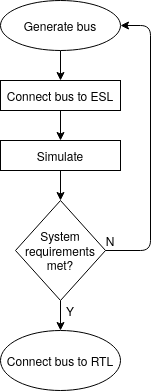
\includegraphics[width=4cm]{figs/Generator.png}
\caption{Design flow with generator}\label{fig:dflow}
\end{wrapfigure}  

The generator takes two input arguments, number of masters and number of slaves. If the input arguments are within the range of 1-15, an ESL and RTL model are generated. After the models are generated, the generator calls the software tool DeSCAM with the SystemC-PPAs of the of the ESL model as input arguments. \par The model is analyzed by the tool and creates and abstract model and property suite. A dedicated plugin uses the abstract model and property suite to create refined property sets and completeness descriptions. The generated models and property files are available in the output folder of the generator. \par A designer can integrate the top-level ESL module of the bus to the system and run simulations. Adding or removing a master or slave require little effort, only a re-run of the generator and a re-integration of the bus into the system. When the system fulfills the requirements, the Property Driven Design flow is followed on the system modules. The developed RTL system modules can be connected to the generated bus without further testing required. The designer can run the property checker Onespin and verify that the bus RTL is a sound abstraction of the bus ESL with a command from the terminal. \par

The following sections describe the bus architecture at the RTL and ESL. chapter.~\ref{ch:design} describes how to recreate the process of developing an abstract ESL model from the RTL, how to generate the system and automatically refine properties.  
\newpage

\section{Register Transfer Level}
\begin{figure}[hbt]
    \begin{center}
        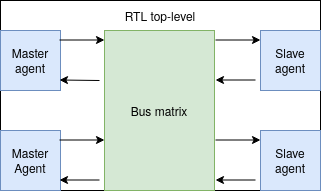
\includegraphics[width=0.8\textwidth]{figs/hw/RTL_top.png}
    \end{center}
    \caption{RTL top-level}
    \label{fig:rtl-top}
\end{figure}

The existing hardware is taken from the \textit{ahb\_system\_generator} found at \\
 www.opencores.com \cite{ahbsys}. This architecture is already structured for the means of generation and is implemented in VHDL, although it does not support wide data bus configurations it is the ideal candidate for this work. The open source architecture has been available for scrutiny online for 15 years and has been referred to by users of hardware forums numerous times when hardware implementations of the AHB is inquired. It is trusted that it adequately complies with the protocol. The architecture includes bus interconnect, address decoder and an arbiter supporting multiple arbitration schemes. The selected arbitration scheme for this work is "fair" fixed-priority. With the "fair" extension, a master which is granted the bus does not lose its grant before its transactions are complete. In other words, early burst termination is disabled. In this work, support for split and retry transfer are not implemented in the agents. Burst transfers are shown as a proof of concept in Sec.~\ref{sec:burst}. The bus interconnect, address decoder and arbiter is grouped in the term "bus matrix", as seen in Fig.~\ref{fig:rtl-top}.\par   

\newpage
\subsection{Master Agent}
\label{sub:magt-rtl}
\begin{wrapfigure}[13]{l}{5cm}
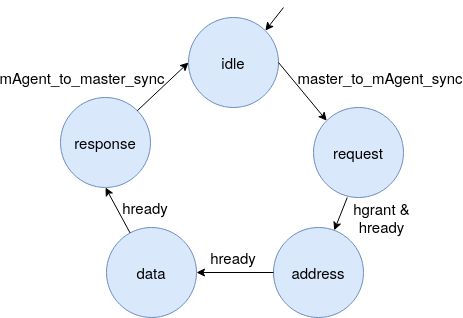
\includegraphics[width=5cm]{figs/hw/mAgent_FSM.png}
\caption{Master agent FSM}\label{fig:rafsm}
\end{wrapfigure}  

The master agent implements the master side of the AHB protocol. It is initialized to the \textit{from\_master} state, where it awaits a payload. The $agent\leftrightarrow master$ interface implements the four phase handshake in both directions. In other words, it is blocked pending a synchronization signal from the master. The payload represents a subset of the AHB master interface, as the remaining signals are either hardwired to default values or modified throughout the transaction. The slave return payload contains a signal which report if the transfer was a success, and valid data if the transaction was a successful read request. An overview of a transfer is provided with respect to the FSM.
\begin{enumerate}
 \item \textit{from\_master}: Initial/idle state, when a synchronization signal is received, the payload is translated to bit and bit vector values and stored in registers.
 \item \textit{Request}: \textbf{HBUSREQx} signals the bus that the agent wants access. The signal remains asserted until the agent is granted access to the bus (\textbf{HGRANTx is set}) and the bus is ready (\textbf{HREADY is set}). When this applies, address and control registers are written to the bus. 
 \item \textit{Address}: \textbf{HTRANS} is encoded with NONSEQ, which signals the slave that a transfer is commencing. This encoding remains on the output until the bus signals that it is ready. When it is ready, data register is written to the bus. 
 \item \textit{Data}: When the bus is ready, return payload is read from the AHB interface and written to the master.
 \item \textit{to\_master}: Agent waits for a synchronization signal from the master. The master should already be asserting its synchronization signal, but this is not a requirement.   
\end{enumerate}

The master agent controls the transfer using \textbf{HBUSREQx} and \textbf{HTRANS}. Conversely, the bus controls the advancement of the transfer phases with \textbf{HREADY} and \textbf{HGRANTx}. The return payload is reported back to the master regardless of transfer direction, reads and writes are therefore not separated within the master agent.  


\newpage
\subsection{Slave agent}
\begin{wrapfigure}[12]{l}{5.5cm}
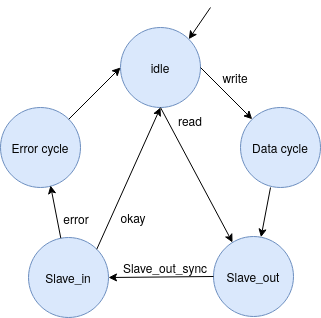
\includegraphics[width=5.5cm]{figs/hw/sAgent_FSM.png}
\caption{Slave agent FSM}\label{fig:rsfsm}
\end{wrapfigure}  

The slave agent implements the slave side of the protocol. The transition conditions in the FSM of Fig.~\ref{fig:rsfsm} are slightly simplified for readability. 
The $agent\leftrightarrow slave$ interface implements a four phase handshake in both directions. Because of this, the slave agent is blocked in the middle of a transfer so it inserts wait states to extend the data phase of the transfer until it the slave has finished processing the request. The payload written to the slave from the agent is equivalent to the payload written from master to agent. An overview of a transaction is given with respect to the FSM.\par
 \vspace{1cm} 

\begin{enumerate}
 \item \textit{idle}: The slave agent remains in this state until it is selected (\textbf{HSELx} is set), the bus is ready and the encoding NONSEQ is detected on \textbf{HTRANS}. When these conditions are true, the slave agent samples address and control signals, drives \textbf{HREADY} low and proceeds to the next state. 
 \item \textit{Data cycle}: If the transaction is a write request an additional cycle is required to sample the data according to protocol. The state advances unconditionally at the next clock edge.
 \item \textit{Slave\_out}: The slave agent signals the slave that the payload is valid by keeping its output notify set. The slave should be ready, but this is not a strict requirement. The slave agent remains in this state, and keeps its notify set until it receives a synchronization signal from the slave.    
 \item \textit{Slave\_in}: The slave agent keeps its input notify set and remains in this state until the request is processed. When the synchronization signal is received, the agent writes response data and transfer status to its bus output registers. 
 \item \textit{Error cycle}: If the transfer status is error, an additional cycle is inserted before returning to idle to provide a two cycle error response. 
\end{enumerate}

The return to idle completes the transfer. The slave agent drives \textbf{HREADY} high and clears the status and response data registers one clock cycle later. 
 

\section{Electronic System Level}
\label{sec:syslev}
\begin{figure}[hbt]
    \begin{center}
        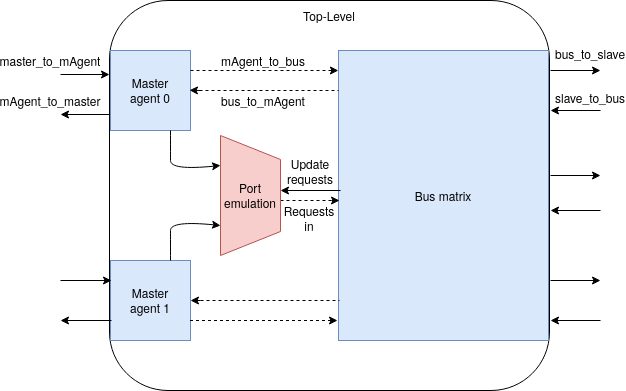
\includegraphics[width=0.8\textwidth]{figs/ESL/syslev_new.png}
    \end{center}
    \caption{ESL top-level}
    \label{fig:esl-top}
\end{figure}

The Electronic System Level models the RTL design described in the previous section. There are no slave agents in the ESL model, but an abstract representation of the master agents remain. Key transfer control signals are modeled with a port emulation module. The port emulation module enable the bus matrix to follow the rules of SystemC-PPA, while providing correct simulation behavior. \WKSAY{Not sure if I should write more about why the port here or if that comes in the design section} 
\newpage

\subsection{Master agent}
\begin{wrapfigure}[10]{l}{5.5cm}
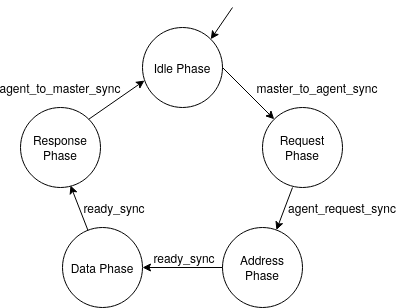
\includegraphics[width=5.5cm]{figs/ESL/mAgent_ESL.png}
\caption{Master agent FSM}\label{fig:eafsm}
\end{wrapfigure}
The FSM of the master agent at the ESL is similar to its RTL counterpart. The control of the transfer flow is accomplished with using a \textit{Blocking} interface in every state. The majority of the AHB master interface signals are represented with the \textit{Shared} interface. Every I/O signal between the master agent and bus matrix that exist in the RTL model, are explicitly represented in the ESL model. An overview of the transfer is given with respect to the FSM. \\
\vspace{0.5cm} 

\begin{enumerate}
 \item \textit{from\_master}: The master agent receives the payload from a blocking\_in port and proceeds to the next state.
 \item \textit{Request}: The master agent requests access to the bus with a blocking\_out port. When the master agent is "unblocked", it writes address and control to a shared\_out port and proceeds to the next state.
 \item \textit{Address}: \textit{htrans} on the shared\_out port is encoded with NONSEQ, and the master agent waits for the bus to be ready by writing to a another blocking\_out port. It writes data to the shared\_out port, encodes \textit{htrans} with IDLE and proceeds to the next state when it is unblocked.
 \item \textit{Data}: The master agent waits for the bus to be ready by writing to the same blocking\_out port. It reads the response payload from a shared\_in port when it is unblocked, and proceeds to the next state. 
 \item \textit{to\_master}: The master agent writes the response payload to the master through a blocking\_out port. 
\end{enumerate} 

All the signals on the AHB interface which are hardwired are assigned those values as the system starts up. 

\newpage
\subsection{Bus matrix}
\label{sub:bus-matrix}
\begin{wrapfigure}[18]{l}{5.5cm}
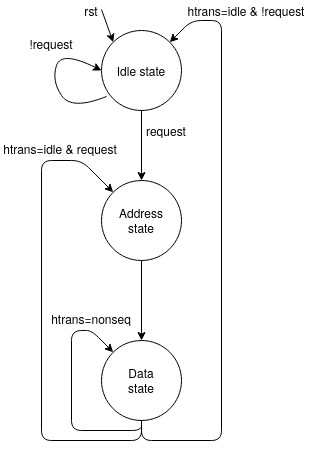
\includegraphics[width=5.5cm]{figs/ESL/Bus_fsm_new.png}
\caption{Bus matrix FSM}\label{fig:busfsm}
\end{wrapfigure}
The bus matrix is described at the ESL with three explicit states. These three states represent the transfer phases only when the transitions $Address\rightarrow Data$ are followed. This is not always the case so it is useful to distinguish the difference between the phases of the transfer and the states of the bus. If the bus is in the state $Address$, there is only one transfer in question and it is in the address phase. If the bus is in the state $Data$, there is one master with its transfer in the data phase, but there may also be a master with its transfer in its address phase. For this reason the word \textit{state} can not be used interchangeably with \textit{phase}, as they could within the master agents.\par
Every I/O signals of the master agent interfaces are represented in the ESL model for all agents. The pipelined behavior of the bus is modeled with the emulated port introduced at the start of this section. A brief overview of the transfer flow is given with respect to the FSM, before each state is described in more detail \par

\begin{enumerate}
 \item \textit{Idle}: The bus matrix fetches updated requests from the port emulation with a non-blocking communication. If there are any pending requests, the payload of the requesting master agent with the highest priority is fetched from a shared\_in port and stored. The bus matrix proceeds to \textit{Address}. 
 \item \textit{Address}: The request payload from the previous state is copied, and the bus fetches updated requests again. The state progresses to \textit{Data} unconditionally.
 \item \textit{Data}: The copied request payload is written to the selected slave through a blocking\_out port, response payload is subsequently read from a blocking\_in port. The response payload is written to all master agents through individual shared\_out ports. Updated requests are again fetched, if there was a request in the previous state, that request payload is copied and this state repeats. If not, the new request payload is stored and the state becomes \textit{Address}. Otherwise the bus becomes idle.    
\end{enumerate}

\subsubsection{Idle}
The process of fetching the updated requests from the emulated port is shown in the following code example. These two ports are the interface between the emulated port and the bus matrix.
\begin{C++}
update_request->try_write(true, sync, "Idle");
requests_in->get(reqs);
\end{C++}
 The process of selecting the appropriate master agent with the fixed priority arbitration scheme is shown with another code example. The fixed-priority arbitration is modeled with an if-else clause, and the chosen master agent payload is fetched from its interface and stored. The ESL model also keeps track of which master owns the address bus. This process occur in every state, with the only difference being the state transitions. 

\begin{C++}
 if(reqs.m0_request){
   mAgent_to_bus0->get(payload0);
   addr_own = 0;
   nextphase = Address;
   AS_regs.haddr = payload0.haddr;
   AS_regs.htrans = nonseq;
   AS_regs.hwrite = payload0.hwrite;
   AS_regs.hsize = payload0.hsize
 }else if(reqs.m1_request){
   mAgent_to_bus1->get(payload1);
   addr_own = 1;
   nextphase = Address;
   AS_regs.haddr = payload1.haddr;
   AS_regs.htrans = nonseq;
   AS_regs.hwrite = payload1.hwrite;
   AS_regs.hsize = payload1.hsize
 }
\end{C++}

All outputs to the master agents are updated in every state.
The signal \textit{hgrant} is functionally represented through \textit{update\_requests}, but is again represented through a shared interface to explicitly represent the complete set of I/O signals. To limit unnecessary overhead, it is represented with an enum rather than specific values.  
\begin{C++}
to_mAgent(x).hresp = ok_resp; 
to_mAgent(x).hrdata = 0; 
to_mAgent(x).hgrant = m(x)_grant;
bus_to_mAgent(x)->set(to_mAgent(x)); 
\end{C++}

		
\subsubsection{Address}
This state does the same as the Idle state, with a few exceptions. Some key values are copied to handle the transition between \textit{Address} and \textit{Data}.

\begin{C++}
DS_regs.haddr = AS_regs.haddr; 
DS_regs.hwrite = AS_regs.hwrite; 
DS_regs.hsize = AS_regs.hsize; 
data_own = addr_own;
\end{C++}

\textit{AS\_regs} are subsequently available for storing the payload of a new requesting master agent. If there are none, the default masters interface is read and assigned. The state transitions unconditionally to \textit{Data}.

\subsubsection{Data}
The variable \textit{DS\_regs.haddr} is used to determine which slave the master agent intends to communicate with. \textit{DS\_regs.hwrite} indicates whether or not the transaction is a write. If the transaction is a write, the payload data of the data bus owner is fetched.
\begin{C++}
if(DS_regs.hwrite == AHB_WRITE){
mAgent_to_bus0->get(payload0);
mAgent_to_bus1->get(payload1);
DS_regs.hwdata = getHwdata(payload0, payload1, data_own);
}else{
DS_regs.hwdata = 0;
}
\end{C++}  

The request is subsequently communicated to the slave. The slave address offset is subtracted and the request is handled by the slave. If the response payload signals error, an error is excplicitly signaled to each master agent.
\begin{C++}
DS_temp.haddr = DS_temp.haddr - slave0_start;
bus_to_slave0->write(DS_temp, "slave_agent0_writes_out");
slave_to_bus0->read(resp, "slave_agent0_reads_back");
\end{C++} 

After the response is written back to the master agents the same process of updating requests as shown in the state \textit{Idle} is carried out, with a slight addition. It is checked if there is a master agent with its transfer in the address phase, if so, the key values are copied as shown for state \textit{Address} and the next state is \textit{Data}. If the address of \textit{DS\_regs.haddr} is not within a valid slave range, an error response is provided.    


\subsection{Port emulation}
\begin{figure}[hbt]
 \centering
 \begin{subfigure}[b]{0.4\linewidth}
 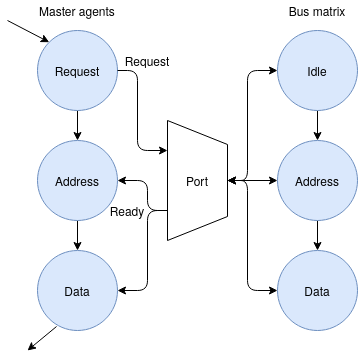
\includegraphics[width=\linewidth]{figs/ESL/port_em.png}
 \caption{Port structure illustrated}
 \end{subfigure}
 \begin{subfigure}[b]{0.3\linewidth}
 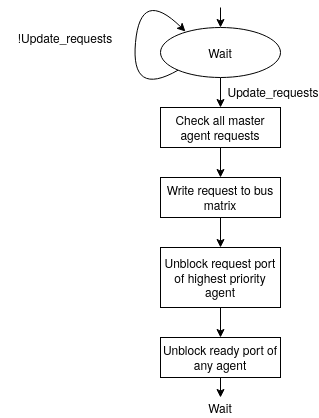
\includegraphics[width=\linewidth]{figs/ESL/port_fsm.png}
 \caption{Port function diagram}
 \end{subfigure}
\caption{Emulated port}
\label{fig:em-port}
\end{figure}


The port emulation is a helper module which is intended to represent the behavior of a non-existent SystemC-PPA port, no properties are generated from this module. It is required to adequately reflect the pipelined behavior of the bus, while simultaneously having a set of properties from the bus matrix which can hold on the design. Fig.~\ref{fig:em-port} a) is a simplified illustration of the port with one master agent connected. All master agents are in fact connected to the same port. \par
The port forwards request from the highest priority master agent to the bus matrix. It unblocks the requesting master with highest priority, and any masters blocked in the address and data phase. All interactions with the master agents are done uninterrupted, in other words no wait statements are called during the process. \par
This port models the signals which control the flow of transfer which were briefly discussed in Sec.~\ref{sub:magt-rtl}. Namely it compresses the functionality of the $agent\leftrightarrow matrix$ interfaces which cover the signals \textbf{HBUSREQx}, \textbf{HREADY} and \textbf{HGRANTx}, so that a single blocking interface covering all agents is available to the bus matrix.






